\documentclass[journal,12pt,twocolumn]{IEEEtran}
\usepackage{setspace}
\usepackage{gensymb}
\singlespacing
\usepackage[cmex10]{amsmath}

\usepackage{amsthm}

\usepackage{mathrsfs}
\usepackage{txfonts}
\usepackage{stfloats}
\usepackage{bm}
\usepackage{cite}
\usepackage{cases}
\usepackage{subfig}

\usepackage{longtable}
\usepackage{multirow}

\usepackage{enumitem}
\usepackage{mathtools}
\usepackage{steinmetz}
\usepackage{tikz}
\usepackage{circuitikz}
\usepackage{verbatim}
\usepackage{tfrupee}
\usepackage[breaklinks=true]{hyperref}
\usepackage{graphicx}
\usepackage{tkz-euclide}

\usetikzlibrary{calc,math}
\usepackage{listings}
    \usepackage{color}                                            %%
    \usepackage{array}                                            %%
    \usepackage{longtable}                                        %%
    \usepackage{calc}                                             %%
    \usepackage{multirow}                                         %%
    \usepackage{hhline}                                           %%
    \usepackage{ifthen}                                           %%
    \usepackage{lscape}     
\usepackage{multicol}
\usepackage{chngcntr}

\DeclareMathOperator*{\Res}{Res}

\renewcommand\thesection{\arabic{section}}
\renewcommand\thesubsection{\thesection.\arabic{subsection}}
\renewcommand\thesubsubsection{\thesubsection.\arabic{subsubsection}}

\renewcommand\thesectiondis{\arabic{section}}
\renewcommand\thesubsectiondis{\thesectiondis.\arabic{subsection}}
\renewcommand\thesubsubsectiondis{\thesubsectiondis.\arabic{subsubsection}}


\hyphenation{op-tical net-works semi-conduc-tor}
\def\inputGnumericTable{}                                 %%

\lstset{
%language=C,
frame=single, 
breaklines=true,
columns=fullflexible
}
\begin{document}


\newtheorem{theorem}{Theorem}[section]
\newtheorem{problem}{Problem}
\newtheorem{proposition}{Proposition}[section]
\newtheorem{lemma}{Lemma}[section]
\newtheorem{corollary}[theorem]{Corollary}
\newtheorem{example}{Example}[section]
\newtheorem{definition}[problem]{Definition}

\newcommand{\BEQA}{\begin{eqnarray}}
\newcommand{\EEQA}{\end{eqnarray}}
\newcommand{\define}{\stackrel{\triangle}{=}}
\bibliographystyle{IEEEtran}
\raggedbottom
\setlength{\parindent}{0pt}
\providecommand{\mbf}{\mathbf}
\providecommand{\pr}[1]{\ensuremath{\Pr\left(#1\right)}}
\providecommand{\qfunc}[1]{\ensuremath{Q\left(#1\right)}}
\providecommand{\sbrak}[1]{\ensuremath{{}\left[#1\right]}}
\providecommand{\lsbrak}[1]{\ensuremath{{}\left[#1\right.}}
\providecommand{\rsbrak}[1]{\ensuremath{{}\left.#1\right]}}
\providecommand{\brak}[1]{\ensuremath{\left(#1\right)}}
\providecommand{\lbrak}[1]{\ensuremath{\left(#1\right.}}
\providecommand{\rbrak}[1]{\ensuremath{\left.#1\right)}}
\providecommand{\cbrak}[1]{\ensuremath{\left\{#1\right\}}}
\providecommand{\lcbrak}[1]{\ensuremath{\left\{#1\right.}}
\providecommand{\rcbrak}[1]{\ensuremath{\left.#1\right\}}}
\theoremstyle{remark}
\newtheorem{rem}{Remark}
\newcommand{\sgn}{\mathop{\mathrm{sgn}}}
\providecommand{\abs}[1]{\left\vert#1\right\vert}
\providecommand{\res}[1]{\Res\displaylimits_{#1}} 
\providecommand{\norm}[1]{\left\lVert#1\right\rVert}
%\providecommand{\norm}[1]{\lVert#1\rVert}
\providecommand{\mtx}[1]{\mathbf{#1}}
\providecommand{\mean}[1]{E\left[ #1 \right]}
\providecommand{\fourier}{\overset{\mathcal{F}}{ \rightleftharpoons}}
%\providecommand{\hilbert}{\overset{\mathcal{H}}{ \rightleftharpoons}}
\providecommand{\system}{\overset{\mathcal{H}}{ \longleftrightarrow}}
	%\newcommand{\solution}[2]{\textbf{Solution:}{#1}}
\newcommand{\solution}{\noindent \textbf{Solution: }}
\newcommand{\cosec}{\,\text{cosec}\,}
\providecommand{\dec}[2]{\ensuremath{\overset{#1}{\underset{#2}{\gtrless}}}}
\newcommand{\myvec}[1]{\ensuremath{\begin{pmatrix}#1\end{pmatrix}}}
\newcommand{\mydet}[1]{\ensuremath{\begin{vmatrix}#1\end{vmatrix}}}
\numberwithin{equation}{subsection}
\makeatletter
\@addtoreset{figure}{problem}
\makeatother
\let\StandardTheFigure\thefigure
\let\vec\mathbf
\renewcommand{\thefigure}{\theproblem}
\def\putbox#1#2#3{\makebox[0in][l]{\makebox[#1][l]{}\raisebox{\baselineskip}[0in][0in]{\raisebox{#2}[0in][0in]{#3}}}}
     \def\rightbox#1{\makebox[0in][r]{#1}}
     \def\centbox#1{\makebox[0in]{#1}}
     \def\topbox#1{\raisebox{-\baselineskip}[0in][0in]{#1}}
     \def\midbox#1{\raisebox{-0.5\baselineskip}[0in][0in]{#1}}
\vspace{3cm}
\title{Assignment 1}
\author{Sudeep Veggalam - EE18BTECH11045}
\maketitle
\newpage
\renewcommand{\thefigure}{\theenumi}
\renewcommand{\thetable}{\theenumi}
\bigskip
Download all the codes from 
\begin{lstlisting}
https://github.com/sudeepv/EE3025_IDP/Assignment1/codes
\end{lstlisting}
and latex-tikz codes from
\begin{lstlisting}
https://github.com/sudeepv/EE3025_IDP/Assignment1
\end{lstlisting}


\section{Digital Filter}
\begin{enumerate}[label=\thesection.\arabic*
,ref=\thesection.\theenumi]
\item
\label{prob:input}
Download the sound file from  
\begin{lstlisting}
wget https://raw.githubusercontent.com/gadepall/EE1310/master/filter/codes/Sound_Noise.wav
\end{lstlisting}
\item
\label{prob:output}
Write the python code for removal of out of band noise and execute the code.
\\
\solution
\lstinputlisting{./codes/cancel_noise.py}
\end{enumerate}


\section{Difference equation}
\begin{enumerate}[label=\thesection.\arabic*,ref=\thesection.\theenumi]
\item
\label{prob:diff_eq}
Write the difference equation of the above Digital filter obtained in problem \ref{prob:output}.
\\
\solution
From \ref{prob:output}, we get,
\begin{equation}
\label{eq:an}
a[n] = \cbrak{\underset{\uparrow}{0.003},0.014,0.021 , 0.0138 ,0.003}
\end{equation}
\begin{equation}
\label{eq:bn}
b[n] = \cbrak{\underset{\uparrow}{1},-2.519,2.561,-1.206,0.220}
\end{equation}
From 
\begin{align}
\label{eq:iir_filter_gen}
 \sum _{m=0}^{M}a\brak{m}y\brak{n-m}=\sum _{k=0}^{N}b\brak{k}x\brak{n-k}
\end{align}
The resultant difference equation is given by \eqref{eq:diff_eqn}
\begin{align}
\label{eq:diff_eqn}
y(n) - 2.52y(n-1) + 2.56y(n-2) - 1.206y(n-3)
\nonumber\\
+ 0.22013y(n-4) = 0.00345x(n) + 0.0138x(n-1) +
\nonumber\\
 0.020725x(n-2) + 0.0138x(n-3) + 0.00345x(n-4)
\end{align}
\item
\label{prob:xnyn_plot1}
Sketch x(n) and y(n).
\\
\solution
The following code writes the .wav file into a .dat file.
\begin{lstlisting}
codes/generate_x.c
\end{lstlisting}
The following C code computes $x(n)$ and $y(n)$ from the difference equation
\begin{lstlisting}
codes/plot_xnyn.c
\end{lstlisting}
The following code plots Fig. \ref{fig:xnyn}
\begin{lstlisting}
codes/plot_xnyn.py
\end{lstlisting}
\begin{figure}[!ht]
\begin{center}
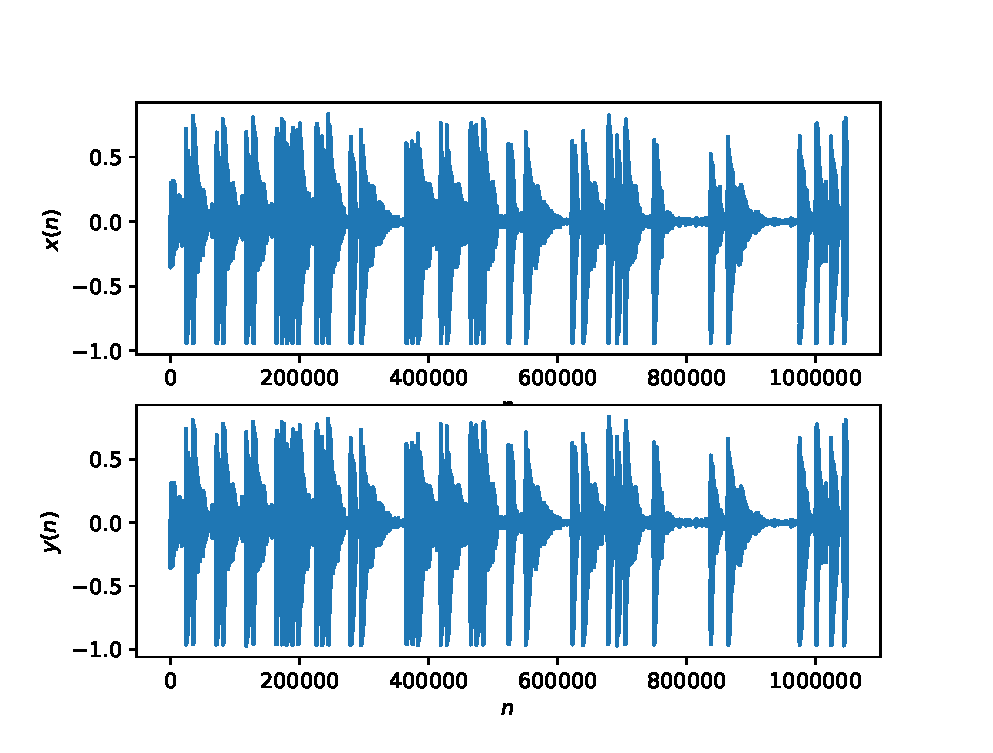
\includegraphics[width=\columnwidth]{./figs/plot_xnyn}
\end{center}
\captionof{figure}{$x(n)$ and $y(n)$ obtained from difference equations}
\label{fig:xnyn}	
\end{figure}
\end{enumerate}



\section{Z-transform}
\begin{enumerate}[label=\thesection.\arabic*,ref=\thesection.\theenumi]
\item
\label{prob:Z-transform_formula}
%
The Z-transform of $x(n)$ is defined as
\begin{align}
\label{eq:z_trans}
X(z)={\mathcal {Z}}\{x(n)\}=\sum _{n=-\infty }^{\infty }x(n)z^{-n}
\end{align}
%
Show that
\begin{equation}
\label{eq:shift1}
{\mathcal {Z}}\{x(n-1)\} = z^{-1}X(z)
\end{equation}
and find
\begin{equation}
	{\mathcal {Z}}\{x(n-k)\} 
\end{equation}
\\
\solution From \eqref{eq:z_trans},
\begin{align}
{\mathcal {Z}}\{x(n-1)\} &=\sum _{n=-\infty }^{\infty }x(n-1)z^{-n}
\\
&=\sum _{n=-\infty }^{\infty }x(n)z^{-n-1} = z^{-1}\sum _{n=-\infty }^{\infty }x(n)z^{-n}
\end{align}
resulting in \eqref{eq:shift1}. Similarly, it can be shown that
%
\begin{equation}
\label{eq:z_trans_shift}
	{\mathcal {Z}}\{x(n-k)\} = z^{-k}X(z)
\end{equation}
\item Find
%
\begin{equation}
H(z) = \frac{Y(z)}{X(z)}
\end{equation}
%
from  \eqref{eq:diff_eqn} assuming that the $Z$-transform is a linear operation.
\\
\solution  From \eqref{eq:z_trans_shift} and \eqref{eq:diff_eqn} we get,
\begin{align}
\begin{split}
H(z) &= \frac{Y(z)}{X(z)}                
\\
&=\frac{b[0]+b[1]z^{-1}+b[2]z^{-2}+b[3]z^{-3}+b[4]z^{-4}}{a[0]+a[1]z^{-1}+a[2]z^{-2}+a[3]z^{-3}+a[4]z^{-4}}
\label{eq:freq_resp}
\end{split}
\end{align}
where a and b are given by \eqref{eq:an} and \eqref{eq:bn}
%
\item 
Let
\begin{equation}
H\brak{e^{\j w}} = H\brak{z = e^{\j w}}.
\end{equation}
Plot $\abs{H\brak{e^{\j w}}}$.
\\
\solution
The following code plots Fig. \ref{fig:H(jw)}.
\begin{lstlisting}
codes/plot_H_jw.py
\end{lstlisting}
\begin{figure}[!ht]
\centering
\includegraphics[width=\columnwidth]{./figs/mag_H(jw)}
\caption{$\abs{H\brak{e^{\j w}}}$}
\label{fig:H(jw)}
\end{figure}
\end{enumerate}



\section{Impulse Response}
\begin{enumerate}[label=\thesection.\arabic*,ref=\thesection.\theenumi]
\item
Sketch h(n).
\label{prob:h(n)}
\\
\solution
$h(n)$ (impulse response) is the output of the system if the unit impulse $\delta(n)$ is given as the input. Substituting $x(n)= \delta(n)$ in Eq. \eqref{eq:diff_eqn}, we get h(n) of the system.

The following C code computes $h(n)$ from the difference equation \eqref{eq:diff_eqn}
\begin{lstlisting}
codes/hn_compute.c
\end{lstlisting}
The following code plots Fig. \ref{fig:h(n)}
\begin{lstlisting}
codes/hn_plot.py
\end{lstlisting}
\begin{figure}[!ht]
\centering
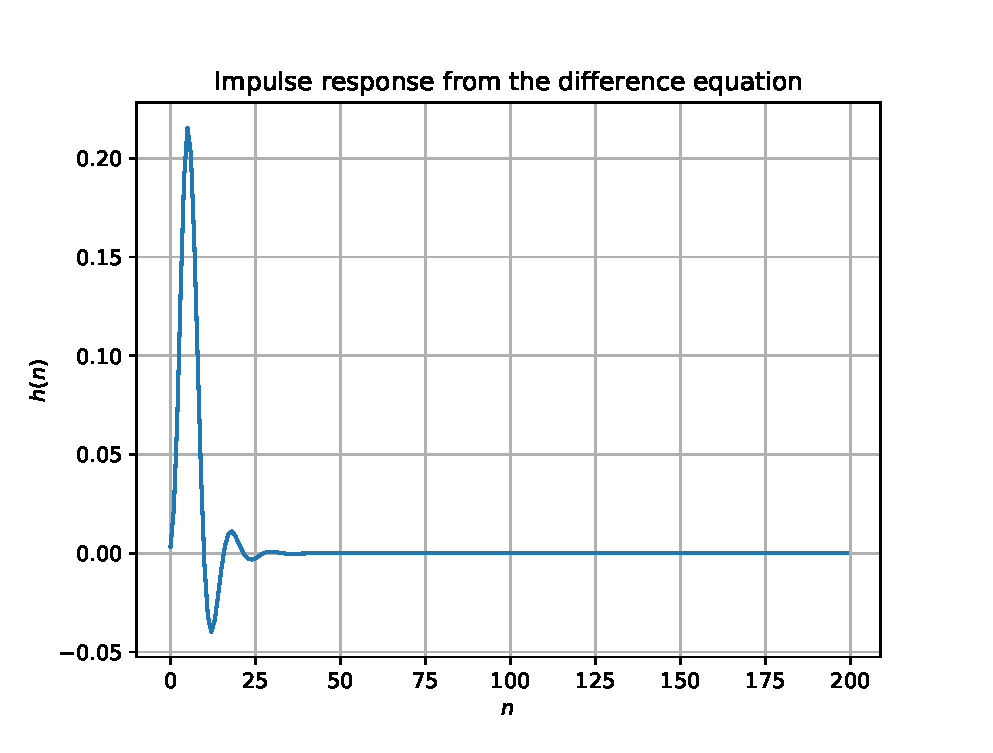
\includegraphics[width=\columnwidth]{./figs/hn}
\caption{Impulse Response ($h(n)$)}
\label{fig:h(n)}
\end{figure}
\item Check whether h(n) obtained is stable.
\\
\solution
From BIBO stability criterion - for a system to be stable, output should be bounded for any bounded input
Since the input x(n) is bounded, if $B_{x}$ is some finite value
\begin{equation}
\abs{y(n)} \leq B_{x}\sum_{-\infty}^{\infty} \abs{x(n-k)}
\label{eq:bibo}
\end{equation}
As y(n) is the convolved output of x(n) and h(n)
\begin{align}
y(n)=h(n) * x(n) = x(n) * h(n)
\end{align}
Equation \eqref{eq:bibo} implies,
\begin{equation}
\abs{y(n)} = \abs{\sum_{-\infty}^{\infty} h(k)x(n-k)}
\end{equation}
\begin{equation}
\abs{y(n)} \leq \sum_{-\infty}^{\infty} \abs{h(k)}\abs{x(n-k)}
\end{equation}
Let $B_{x}$ be the maximum value x(n-k) can take, then
\begin{equation}
\abs{y(n)} \leq B_{x}\sum_{-\infty}^{\infty} \abs{h(k)}
\end{equation}
If
\begin{equation}
\sum_{-\infty}^{\infty} \abs{h(k)} < \infty
\end{equation}
Then
\begin{equation}
\abs{y(n)} \leq B_{y} < \infty
\end{equation}
Therefore we can say that y(n) is bounded if x(n) and h(n) are bounded.
Since the audio input is bounded, the system is said to be stable if h(n) is also bounded
\begin{equation}
\sum_{n=-\infty}^{n=-\infty} \abs{h(n)}<\infty
\end{equation}
The above equation can be re written as,
\begin{equation}
\sum_{n=-\infty}^{n=\infty} \abs{h(n)z^{-n}}_{\abs{z}=1}<\infty
\end{equation}
\begin{equation}
\sum_{n=-\infty}^{n=-\infty} \abs{h(n)} \abs{z^{-n}}_{\abs{z}=1}<\infty
\end{equation}
From Triangle inequality,
\begin{equation}
\abs{\sum_{n=-\infty}^{n=-\infty} h(n)z^{-n}}_{\abs{z}=1}<\infty
\end{equation}
\begin{equation}
\implies \abs{H(z)}_{\abs{z}=1} < \infty
\end{equation}
For the system to be stable, the Region of Convergence(ROC) should include the unit circle.
Since, h(n) is right sided the ROC is outside the outer most pole. The following code computes the poles of the transfer function given by \eqref{eq:freq_resp}
\begin{lstlisting}
codes/compute_poles.py
\end{lstlisting}
Poles of the given transfer equation are:
\begin{equation}
\begin{split}
z(approx) = 0.69786079 \pm 0.41316978j,
\\
0.56187146 \pm 0.13779107j
\end{split}  
\end{equation}
From the above poles, we can see that that the ROC of the system is
\begin{align}
\abs{z}&> max(\sqrt{0.69^{2}+0.41^{2}},\sqrt{0.56^{2}+0.13^{2}})
\\
\abs{z}&> max(0.811,0.578)
\\
\abs{z}&> 0.811
\label{eq:roc}
\end{align}

From \eqref{eq:roc}, ROC of the system includes unit circle $\abs{z}=1$. Therefore, the given IIR filter is stable, since h(n) is absolutely summable.
\\
\textbf{Verification}:-
Given bounded input x(n) (audio sample) and system difference equation \eqref{eq:diff_eqn}
From Fig. \ref{fig:xnyn} we can see that the maximum value of x(n) is 0.8311 and minimum value is around -0.9417.
Similarly from Fig. \ref{fig:xnyn} we can also observe that the maximum value of y(n) is 0.8362 and minimum value is -0.97 and it tends to zero after the length of signal.
We can conclude that for the bounded input x(n), the output
y(n) is bounded. Therefore, the system is BIBO stable.
\\
\item Compute filtered output using convolution formula with h(n) obtained in \ref{prob:h(n)}
%
\begin{equation}
\label{eq:convolution}
y(n) = x(n)*h(n) = \sum_{n=-\infty}^{\infty}x(k)h(n-k)
\end{equation}
\solution The following code plots Fig. \ref{fig:yn_conv} where $y(n)$ is computed using convolution.
%
\begin{lstlisting}
codes/conv_plot.py
\end{lstlisting}
\begin{figure}[!ht]
\centering
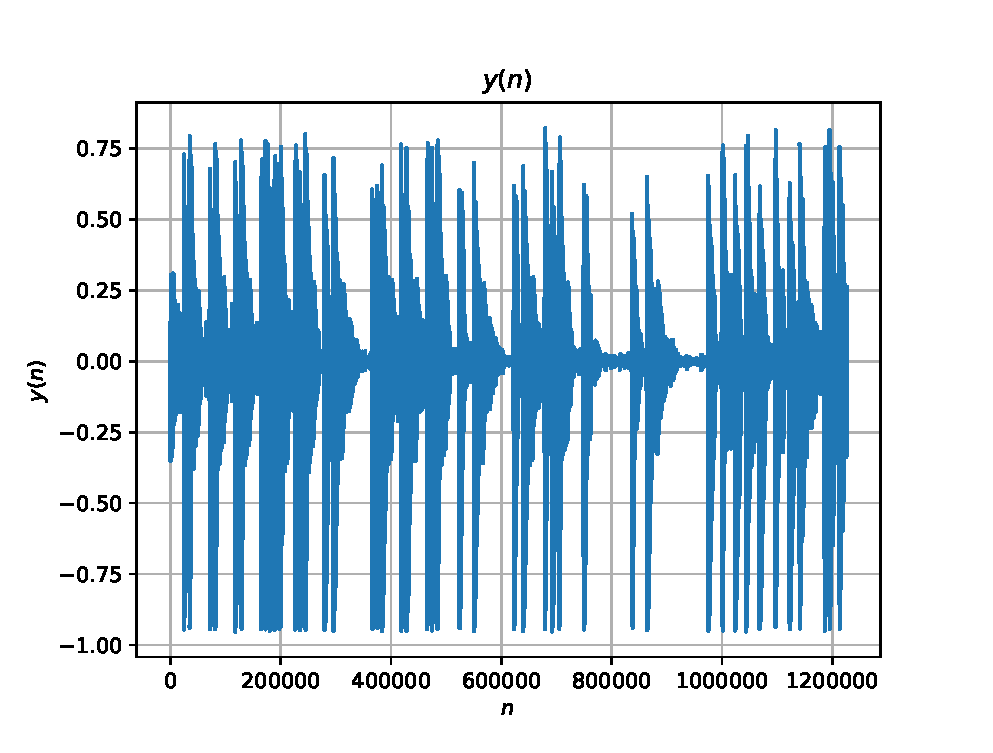
\includegraphics[width=\columnwidth]{./figs/yn_conv}
\caption{$y(n)$ through convolution}
\label{fig:yn_conv}
\end{figure}
We can observe that the output obtained in the Fig. \ref{fig:yn_conv} is same as y(n) obtained in Fig. \ref{fig:xnyn}.
\end{enumerate}



\section{FFT and IFFT}
\begin{enumerate}[label=\thesection.\arabic*
,ref=\thesection.\theenumi]
\item Compute
\begin{align}
        X(k) \triangleq \sum_{n=0}^{N-1} x(n) e^{-j 2 \pi k n / N}, \quad k=0,1, \ldots, N-1
\end{align}
and $H(k)$ using h(n).
\\
\solution
The audio sample x(n) has been obtained in \ref{prob:xnyn_plot1} and the impulse response h(n) has been obtained in \ref{prob:h(n)} 
DFT of the Input Signal $x(n)$ is 
\begin{align}
    X(k) \triangleq \sum_{n=0}^{N-1} x(n) e^{-j 2 \pi k n / N}, \quad k=0,1, \ldots, N-1
\end{align}
DFT of the Impulse Response $h(n)$ is 
\begin{align}
    H(k) \triangleq \sum_{n=0}^{N-1} h(n) e^{-j 2 \pi k n / N}, \quad k=0,1, \ldots, N-1
\end{align}
The following C code computes DFT of $x(n)$ and $h(n)$ efficiently using fft algorithm. It also computes IFFT of Y(k) and creates a .dat file.
\begin{lstlisting}
codes/fft.c
\end{lstlisting}
The following code plots FFTs of $x(n)$ and $h(n)$.
\begin{lstlisting}
codes/fft_plot.py
\end{lstlisting}
Magnitude plots of $|X(k)|$ and $|H(k)|$
\begin{figure}[!ht]
\centering
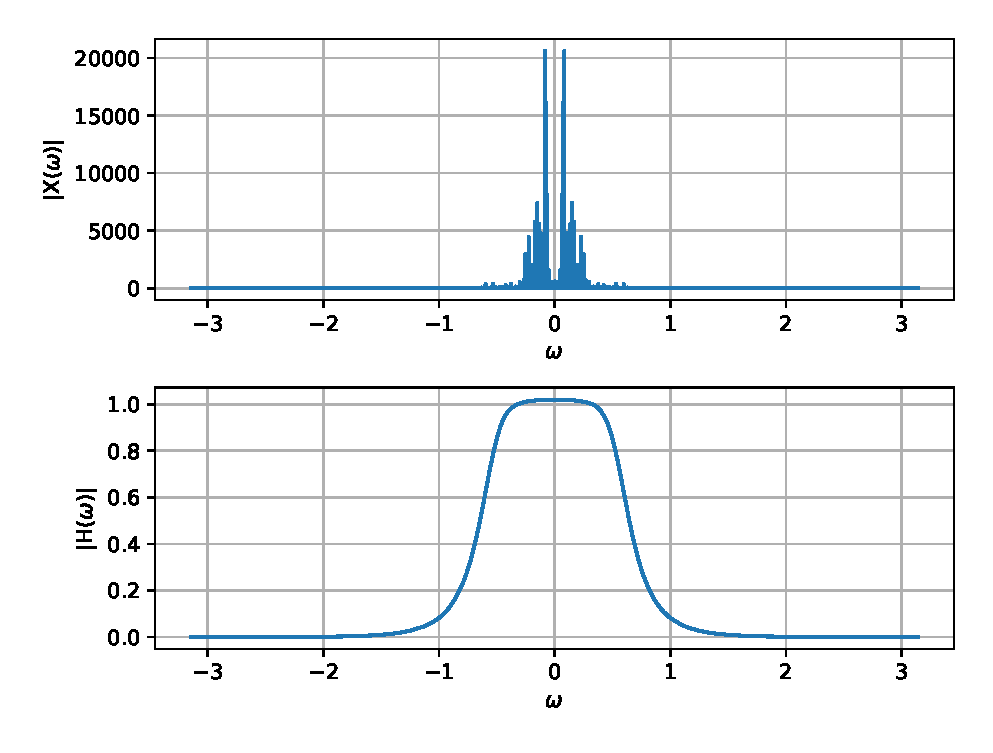
\includegraphics[width=\columnwidth]{./figs/fft}
\caption{$X(k) and H(k)$}
\label{fig:xnhnfft}
\end{figure}
\item From
\begin{equation}
Y(k) = X(k)H(k)
\end{equation}
Compute
\begin{equation}
y(n) \triangleq \sum_{k=0}^{N-1} Y(k) e^{j 2 \pi k n / N}, \quad n=0,1, \ldots, N-1
\end{equation}
\\
\solution
The following code computes the DFT of $y(n)$ by multiplying $X(\omega)$ and $H(\omega)$ and subsequently computes inverse DFT of $Y(\omega)$ to get $y(n)$.
\begin{lstlisting}
codes/ifft.py
\end{lstlisting}
The following code plots $y(n)$.
\begin{lstlisting}
codes/ifft_plot.py
\end{lstlisting}
\begin{figure}[!ht]
\centering
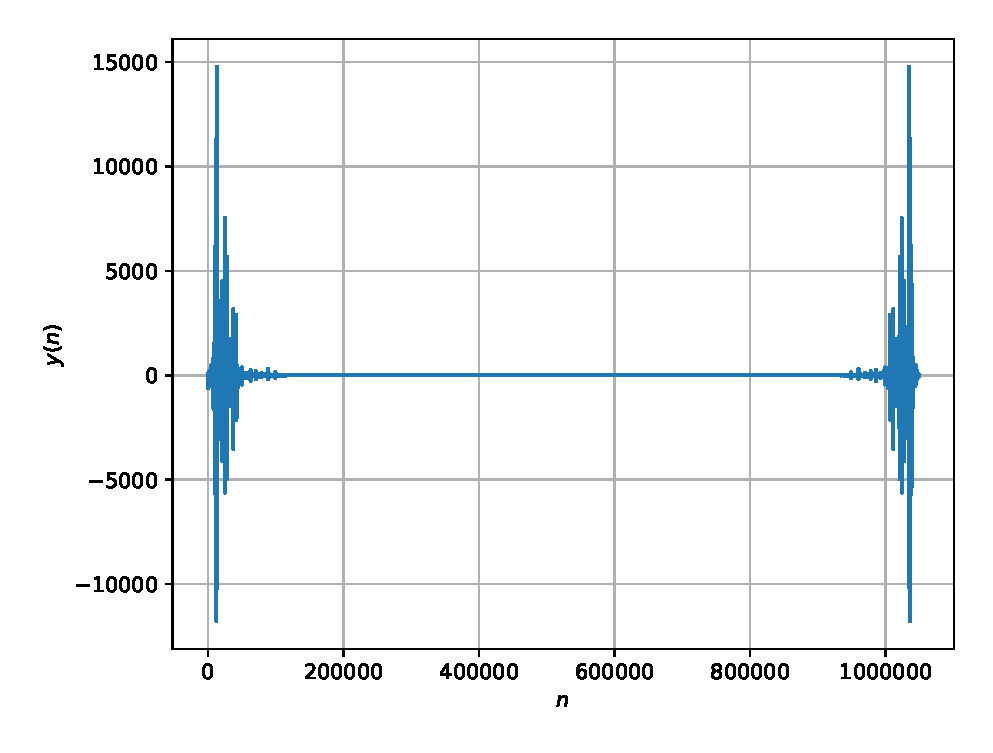
\includegraphics[width=\columnwidth]{./figs/ifft}
\caption{$y(n) through ifft$}
\label{fig:ynfft}
\end{figure}
We can observe from the Fig. \ref{fig:ynfft} that it is same as the y(n) observed in Fig.\ref{fig:xnyn}
\end{enumerate}
\end{document}